\appendix
\section{Supplementary Material}


\subsection{Automated Right Whale Localizer and Segmeneter}
\label{sup:auto_croping}

\begin{figure}[H]
	\centering
	\begin{subfigure}[b]{0.25\linewidth}
		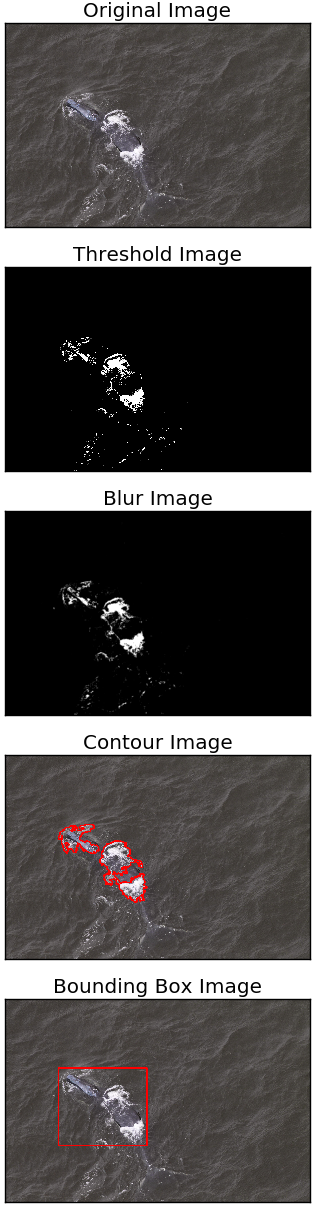
\includegraphics[width=\linewidth]{sections/imgs/preprocessing/figure_1.png}
		\caption{}
	\end{subfigure}
	\begin{subfigure}[b]{0.25\linewidth}
		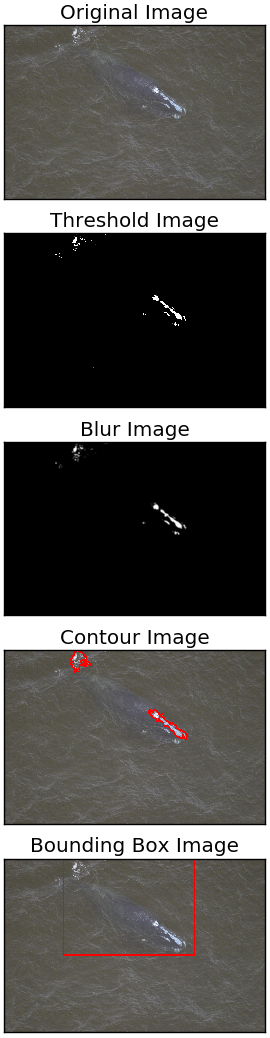
\includegraphics[width=\linewidth]{sections/imgs/preprocessing/figure_2.png}
		\caption{}
	\end{subfigure}
	\begin{subfigure}[b]{0.2515\linewidth}
		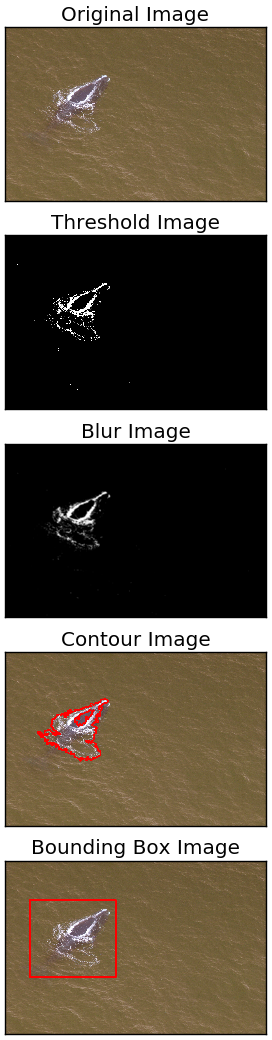
\includegraphics[width=\linewidth]{sections/imgs/preprocessing/figure_3.png}
		\caption{}
	\end{subfigure}
	
	\caption{Automated Right Whale Head Cropping Process}
	\label{fig:auto_head_croper}
\end{figure}

Figure~\ref{fig:auto_head_croper} displays the best case scenario how the automated whale head cropper we implemented was capable of localizing and segmenting the whale head properly, using simple techniques such as thresholding, bluring, contour finding and then cropping by creating a bounding box of the contours found.

\begin{figure}[H]
	\centering
	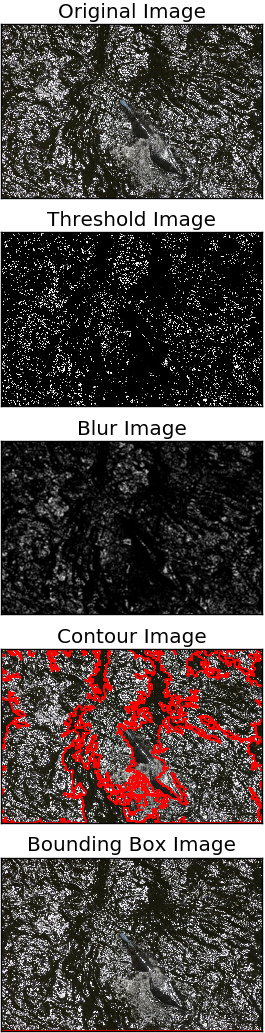
\includegraphics[width=0.3\textwidth]{sections/imgs/preprocessing/worst_case.png}
	\caption{Trouble processing noisy images}
	\label{fig:noisy_data}
\end{figure}

Figure~\ref{fig:noisy_data} show cases the worst case scenario for the automated whale head cropper. As seen in the figure, thresholding fails to mitigate the noise and localize the whale from the image. With the dataset given there were a large portion of images that were as noisy as figure shown.



\subsection{Multi-Layer Perceptron Experiements}
\label{sup:mlp_experiments}

\begin{figure}[H]
	\centering
	\begin{subfigure}[b]{0.45\linewidth}
		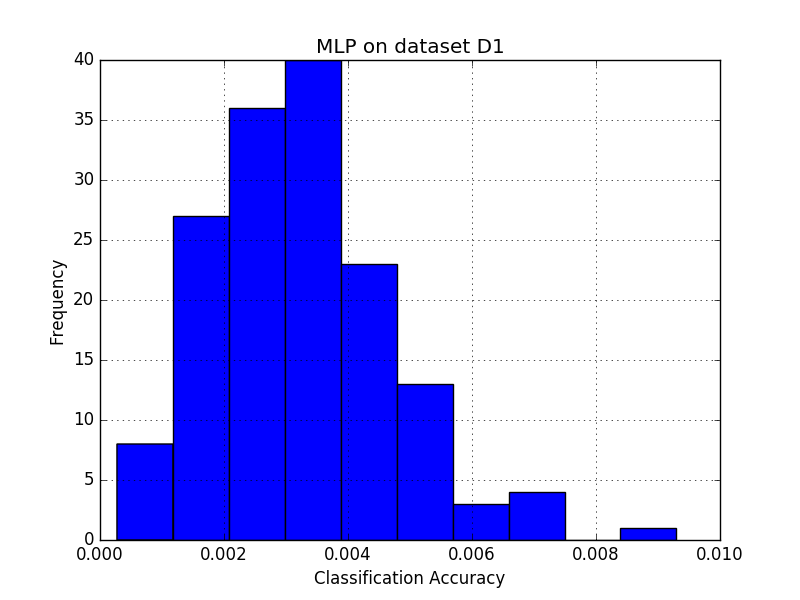
\includegraphics[width=\linewidth]{sections/imgs/mlp/mlp_d1.png}
		\caption{MLP Classification Accuracy on $D_{1}$}
		\label{fig:mlp_d1}
	\end{subfigure}
	\begin{subfigure}[b]{0.45\linewidth}
		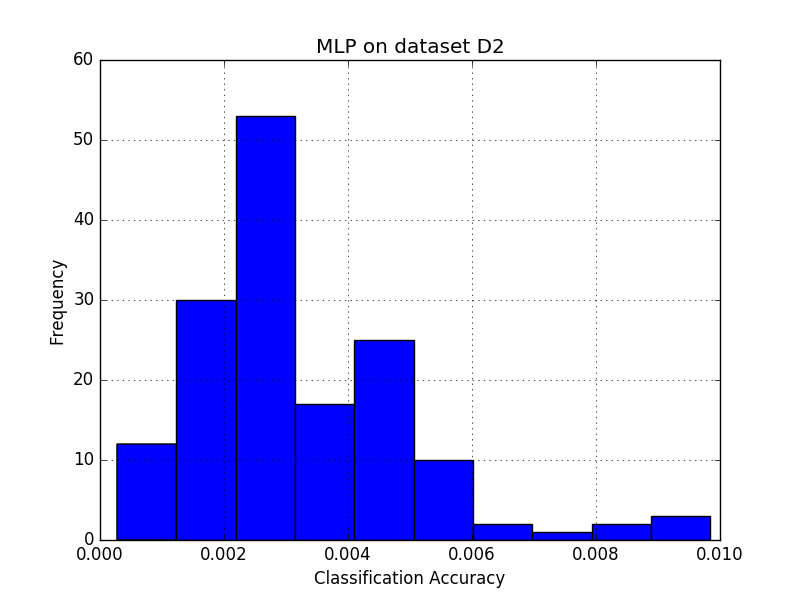
\includegraphics[width=\linewidth]{sections/imgs/mlp/mlp_d2.png}
		\caption{MLP Classification Accuracy on $D_{2}$}
		\label{fig:mlp_d1}
	\end{subfigure}
\end{figure}

As you can see MLP performed very poorly on dataset $D_{1}$, $D_{2}$. We did not continue using MLP for other datasets because we did not find value in doing so.


\subsection{Genetic Algorithm Tuner}
\label{sup:genetic_encoding}
A Genetic Algorithm Tuner was used to attempt to find hyperparameters for deep neural networks. The bit string of an individual represents the hyperparameters of a network. For example if we have a bit string of length 10. The first 3 bits would represent the number of hidden layers (0 - 8: $2^{3}$), and the activation functions would be represented by 2 bits, and so on.

Below details the hyperparameters tuned by the Genetic Algorithm in Section~\ref{sec:tuning_deep_nets_with_ga}.

\subsubsection{Feed-Forward Network Hyperparameters Tuned}
\label{sup:feed_forward_hyperparameters}
For creating hyperparameters for a Feed-Forward Network a custom genetic encoding was devised. A bit string of length 500 was chosen, where the following hyperparameters were tuned with a GA:

\begin{itemize}
	\vspace{-0.5cm}
	\setlength{\itemsep}{0pt}
	\setlength{\parskip}{0pt}
	\setlength{\parsep}{0pt}
	
	\item{No. of Hidden Layers (0 - 8)}
	\item{No. of Hidden Neurons at each layer (0 - 8)}
	\item{Activations used at each layer (sigmoid, tanh, softmax, relu, linear)}
	\item{Dropouts percentages (0\% - 49\%)}
	\item{Optimizer (Adagrad, Ada delta, RMS, SGD)}
	\item{No. of Epoch (0 - 127)}
	\item{Batch Size (0 - 256)}
\end{itemize}


\subsubsection{CNN Hyperparameters Tuned}
\label{sup:cnn_hyperparameters}
The hyperparameters for a CNN network are similar to a Feed-Forward, however there is an architecture constraint. The architecture is as follows, first there are Convolution Layers, followed by a Maxpool layer, at each Maxpool layer there is an option for whethere dropouts are applied, at no point can there be a Maxpool layer before a Convolutional layer. At the end of the combination of Convolution and Maxpool layers is a feed forward network, this acts as the classification network commonly called the softmax network. Below are the hyperparameters tuned:

\begin{itemize}
	\vspace{-0.5cm}
	\setlength{\itemsep}{0pt}
	\setlength{\parskip}{0pt}
	\setlength{\parsep}{0pt}
	
	\item{No. of Convolution Layers (0 - 8)}
	\item{No. of Filters at each Convo layer (0 - 64)}
	\item{Convo Filter Size at each Convo layer (0 - 8)}
	\item{Activations used at each Convo layer (sigmoid, tanh, softmax, relu, linear)}
	\\
	
	\item{Maxpool layer after each Convo layer (true, false)}
	\item{Maxpool Pool Size for each Maxpool layer (0 - 8)}
	\item{Dropouts percentages after each Convo Layer (0\% - 49\%)}
	\\
	
	\item{No. of Feed-Forward Hidden Layers (0 - 8)}
	\item{No. of Feed-Forward Hidden Neurons at each layer (0 - 8)}
	\item{Activations used at each Feed-Forward layer (sigmoid, tanh, softmax, relu, linear)}
	\item{Dropouts percentages at each Feed-Forward Layer (0\% - 49\%)}
	\\
	
	\item{Optimizer (Adagrad, Ada delta, RMS, SGD)}
	\item{No. of Epoch (0 - 127)}
	\item{Batch Size (0 - 256)}
\end{itemize}


\subsection{Genetic Operators}
\label{sup:genetic_operators}
Genetic operators for Gentic Algorithms(GA) is not limited to tournament selection, point crossover and multiple point mutation chosen in Section~\ref{sec:tuning_deep_nets_with_ga}, there exists other operators that might be more suitable for a specific problem, these operators were chosen simply based on intuition and experience. Below we will briefly describe how the chosen genetic operators work discussed in Section~\ref{sec:tuning_deep_nets_with_ga} work.


\subsubsection{Tournament Selection}
Tournament Selection proposed by \cite{miller1995genetic} is a selection method where it creates a tournament size $t$ of randomly selected individuals from the population. The winner of the (one with best fitness) tournament is selected for crossover. There are two types of tournament selection, a deterministic version where the best invidual in the tournament is selected ($p = 1$), or a probabilistic version where the individual has a probability $p (1 - p)^{n}$  where $n$ is the rank of the individual.


\subsubsection{Point Crossover}
\begin{wrapfigure}{L}[0pt]{0.45\textwidth}
	\vspace{-0.4cm}
	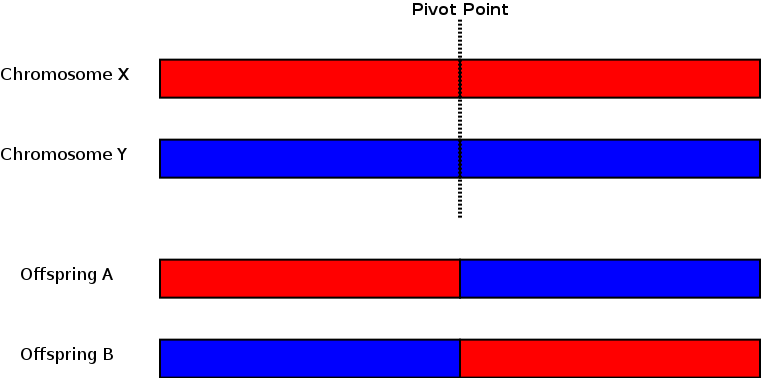
\includegraphics[width=\linewidth]{sections/imgs/ga/ga_crossover.png}
	\caption{Point Crossover}
	\label{fig:ga_point_crossover}
	\vspace{-0.9cm}
\end{wrapfigure}

Point crossover is a standard genetic operator that mimicks biological crossover \cite{mitchell1998introduction}. The operator takes two chromosomes selected by the chosen selection operator as inputs, where a chromosome is an individual in the GA population representing a potential solution to the problem. The operator has a probability $P_{c}$ that will act on chromosome X and Y, where the pivot point forms the point of which different halves of the chromosome are swaped with each other (see Fig~\ref{fig:ga_point_crossover}).

\newpage
\subsubsection{Multiple Point Mutation}
\begin{wrapfigure}{L}[0pt]{0.45\textwidth}
	\vspace{-0.2cm}
	
	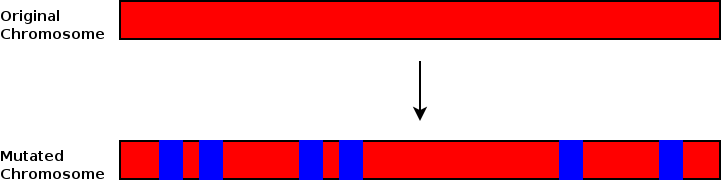
\includegraphics[width=\linewidth]{sections/imgs/ga/ga_multiple_point_mutation.png}
	\caption{Multiple Point Mutation}
	\label{fig:ga_multiple_point_mutation}

	\vspace{-0.5cm}
\end{wrapfigure}

The Multiple point mutation is another genetic operator that mimicks biological mutation \cite{mitchell1998introduction}. The goal is to encourage population diversity by randomly mutating the chromosome's genes. For the multiple point mutation it has a probability $P_{m}$ multiple random points are selected and modified. For a bit string encoding, the bits are given a probability to bit flip.


\subsection{The Evaluation Function in the Genetic Algorithm CNN Tuner}
\label{sup:ga_cnn_tuner_eval_func}
From Section~\ref{sec:ga_cnn_tuner} we discussed how during tuning we were met with an implementation problem, below is the source code listing of the evaluation function which was used by the GA CNN tuner. Of particular interest is between lines 53 to 66, where you can clearly see that the evaluation of the CNN network is encapsulated with a try-catch code block, catching any exceptions that may occur during the evaluation stage. This however did not prevent the code from exiting early while evaluating a CNN network which we found peculiar, we suspect there is a bug in the library we were using.

\begin{lstlisting}[language=Python, caption="Evaluation Function of the GA CNN Tuner"]
def evaluate_cnn(eval_data):
	individual = eval_data["individual"]
	nn_data = eval_data["nn_data"]
	score_cache = eval_data["score_cache"]
	error_cache = eval_data["error_cache"]
	X_train = nn_data["X_train"]
	Y_train = nn_data["Y_train"]
	X_test = nn_data["X_test"]
	Y_test = nn_data["Y_test"]
	input_shape = nn_data["input_shape"]
	n_outputs = nn_data["n_outputs"]
	
	# just to stop syntax checker complaining vars not being used
	X_train
	Y_train
	X_test
	Y_test
	
	# check cache
	chromo_str = "".join(map(str, individual["chromosome"]))
	if chromo_str in score_cache:
		print " in cache! score is: {1}".format(
			chromo_str,
			score_cache[chromo_str]
		)
		score = score_cache[chromo_str]
		individual["score"] = score
		return False
	
	# create folder
	global EVALUATION_COUNTER
	model_save_dir = nn_data["model_save_dir"]
	model_path = os.path.join(
		model_save_dir,
		"model_{0}".format(EVALUATION_COUNTER)
	)
	os.mkdir(model_path)
	EVALUATION_COUNTER += 1
	
	# mapping
	kwargs = mapping.keras_mapping2(individual)
	kwargs["X_train"] = X_train
	kwargs["Y_train"] = Y_train
	kwargs["X_test"] = X_test
	kwargs["Y_test"] = Y_test
	kwargs["input_shape"] = input_shape
	kwargs["nb_classes"] = n_outputs
	kwargs["model_file"] = os.path.join(model_path, "model.json")
	kwargs["weights_file"] = os.path.join(model_path, "weights.dat")
	kwargs["results_file"] = os.path.join(model_path, "results.dat")
	
	# evaluate CNN
	try:
		results, model_score = cnn.cnn(**kwargs)
		print("[score: {0}]".format(model_score[1]))
		
		individual["score"] = model_score[1]
		score_cache[chromo_str] = model_score[1]
		error_cache[chromo_str] = model_score[0]
	
	except Exception:
		print "[failed]"
		if DEBUG:
			import traceback
			traceback.print_exc()
		score = -1

	return True
\end{lstlisting}

\subsection{CNN configurations and experimental results}
\label{sup:cnn_config_result}

\begin{table}[H]
	\begin{center}
	\begin{tabular}{|c|c|c|c|c|}
	\hline
	A & B & C & D & E \\
	\hline
	conv3-32 + max & conv3-32 & conv5-32 + max & conv3-32 + max & conv3-32 + max + dropout \\
	\hline
	conv3-64 + max & conv5-64 + max & conv5-64 + max & conv3-64 & conv3-64 + max + dropout \\
	\hline
	conv3-128 + max & conv5-128 + max & conv3-128 + max & conv3-64 + max & conv3-128 + max + dropout \\
	\hline
	- & conv3-128 + max & - & conv3-128 & - \\
	\hline
	- & - & - & conv3-128 + max & - \\
	\hline
	\multicolumn{5}{|c|}{FC-1000}\\
	\hline
	FC-1000 & FC-1000 & - & FC-1000 & FC-1000 \\
	\hline
	\multicolumn{5}{|c|}{FC-447}\\
	\hline
	\end{tabular}
	\end{center}
	\caption{Architecture specifics for five different CNNs. The convolutional layer parameters are denoted as \lq\lq conv(receptive field size)-(number of channels)\rq\rq. The fully-connected layer parameter is denoted as \lq\lq FC-(number of neurons)\rq\rq}
	\label{cnn_table}
\end{table}

The CNN configurations, evaluated in this project, are outlined in Table~\ref{cnn_table}. Note that ReLU is used in all layers and \lq\lq dropout\rq\rq is applied after all fully-connected layers. The CNN with configuration C is the only one that use one fully-connected layer. It takes the shortest time to train, while has the worst overfitting problem. For dataset $D_{2}$, we test three configurations and get the test accuracy of 10\% approximately. For dataset $D_{3}$, Config B and D give us the best results around 25\%, since they have more layers. We add \lq\lq dropout\rq\rq after convolutional layers in Config E, but it needs too much time for training and the improvement is not as good as expected.

\begin{figure}[H]
	\centering
	\begin{subfigure}[b]{0.4\linewidth}
		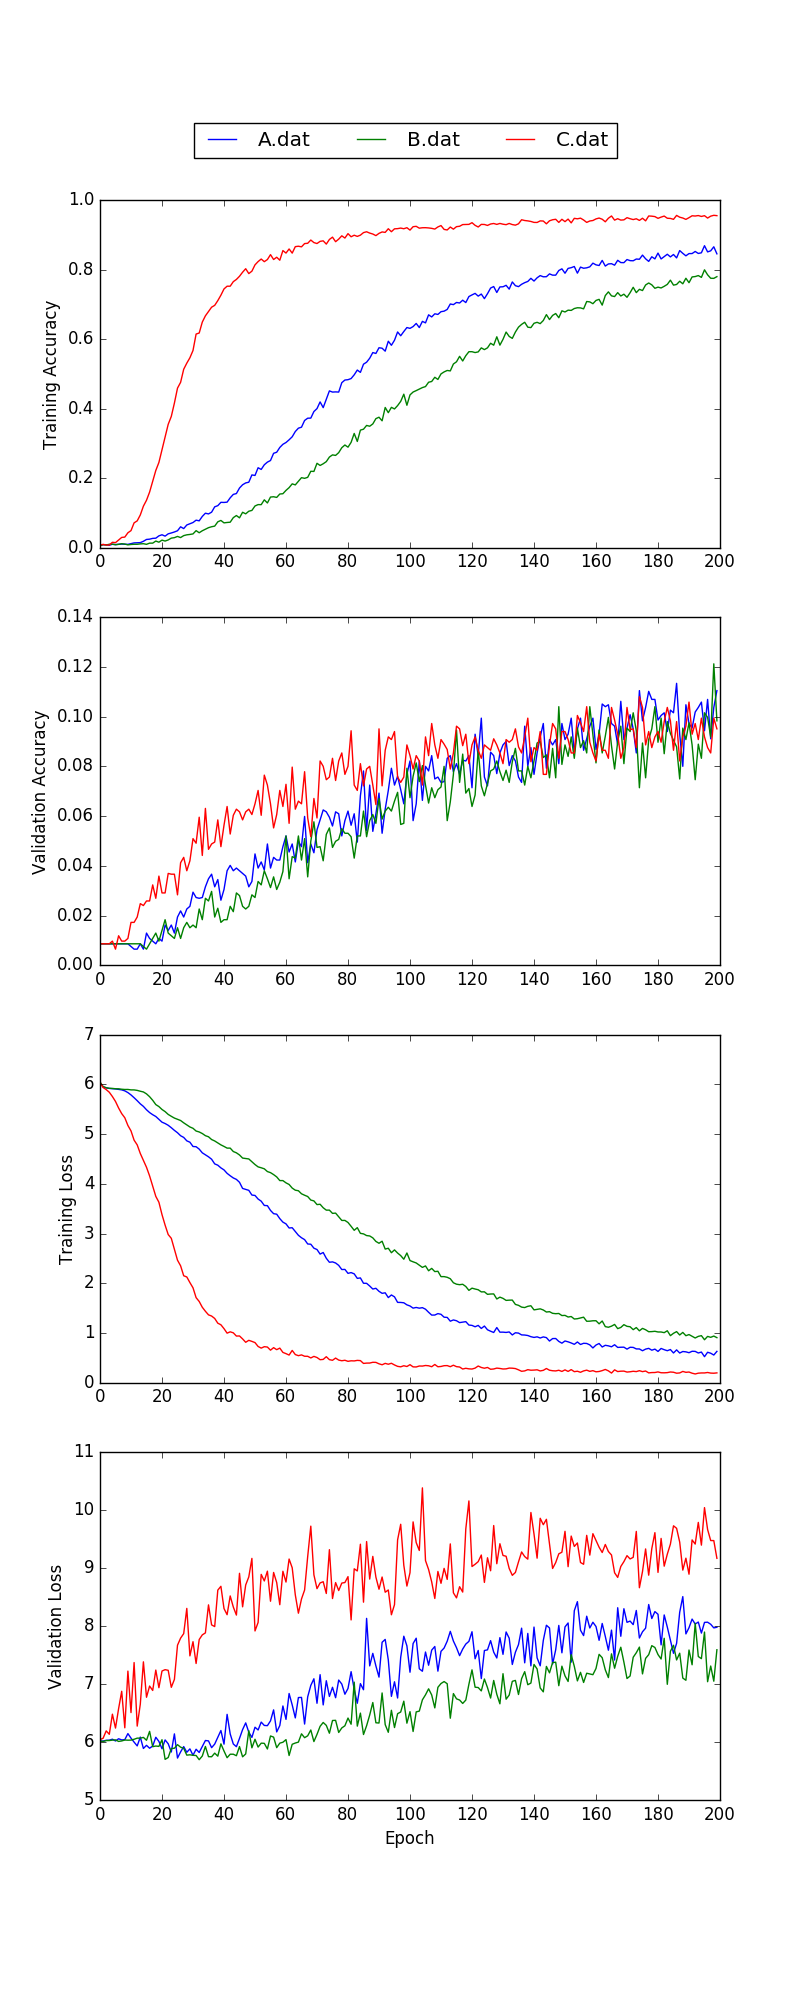
\includegraphics[width=\linewidth]{sections/imgs/cnn/cnn_dataset2.png}
		\caption{CNN experiments on dataset $D_{2}$}
		\label{fig:cnn_d2}
	\end{subfigure}
	\begin{subfigure}[b]{0.4\linewidth}
		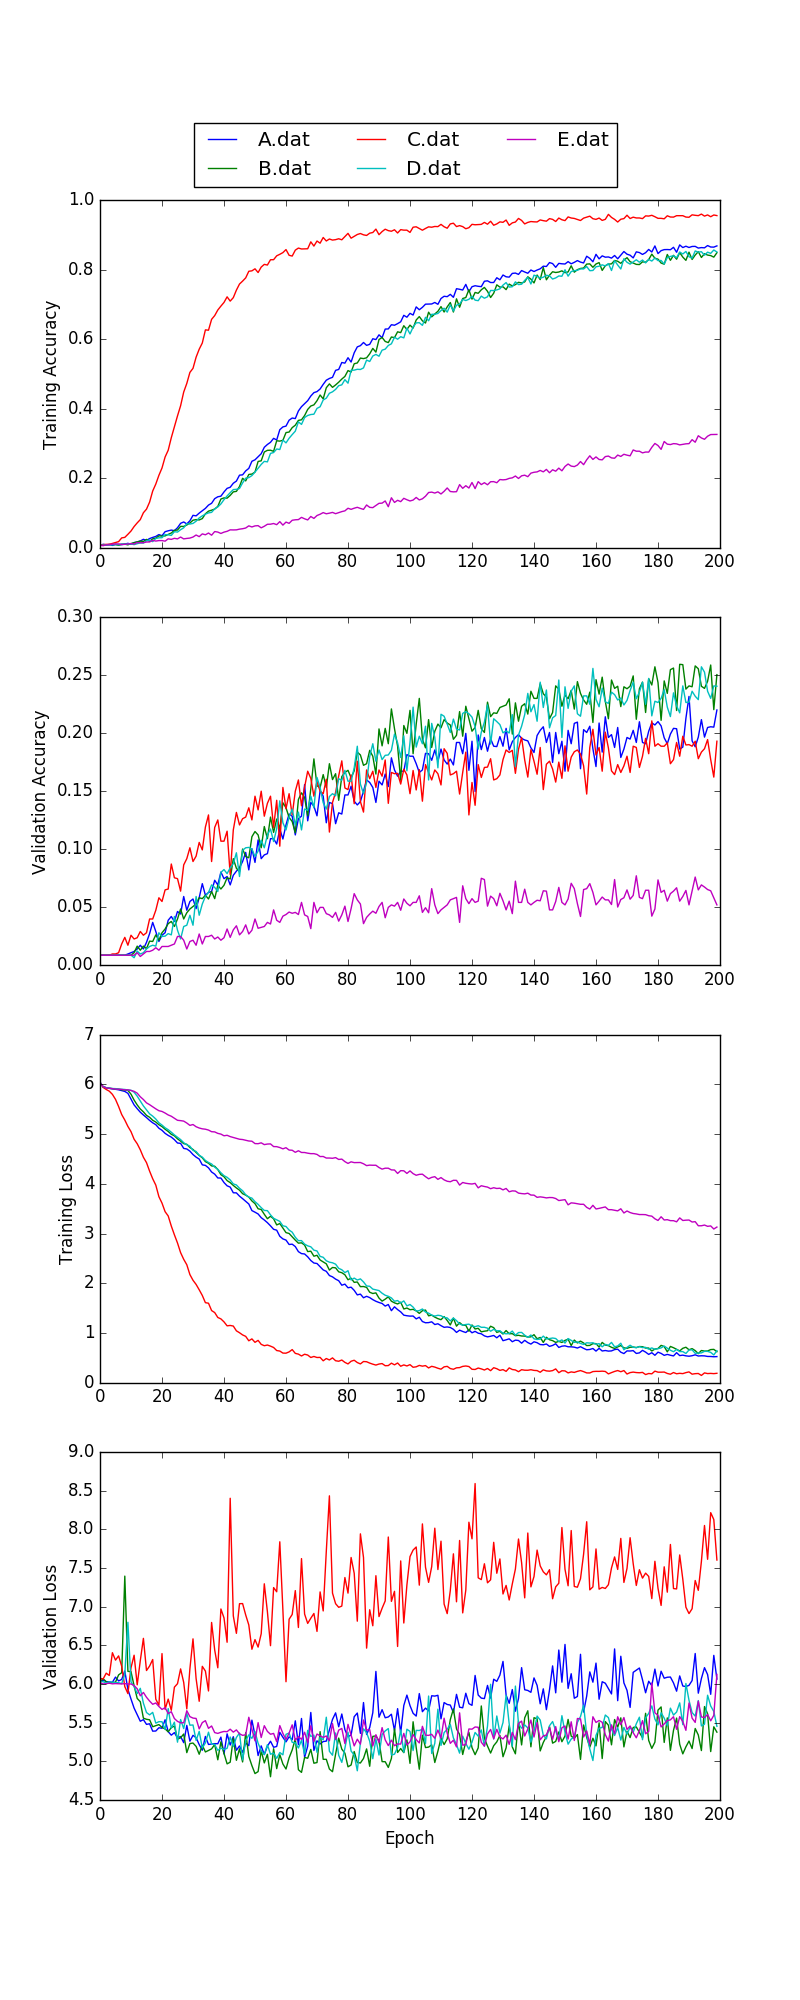
\includegraphics[width=\linewidth]{sections/imgs/cnn/cnn_dataset3.png}
		\caption{CNN experiments on dataset $D_{3}$}
		\label{fig:cnn_d3}
	\end{subfigure}
	
	\caption{CNN experiments on datasets $D_{2}$ and $D_{3}$}
\end{figure}